\documentclass[aspectratio=169]{beamer}

\usetheme{Madrid}
\usecolortheme{default}

\usepackage[utf8]{inputenc}
\usepackage[T1]{fontenc}
\usepackage[english]{babel}
\usepackage{amsmath, amssymb}
\usepackage{graphicx}
\usepackage{hyperref}
\usepackage{listings}
\usepackage{xcolor}
\usepackage{tikz}
\usetikzlibrary{shapes.geometric, arrows.meta, positioning, calc}

% Python style
\lstdefinestyle{python}{
    language=Python,
    basicstyle=\ttfamily\scriptsize,
    keywordstyle=\color{blue}\bfseries,
    stringstyle=\color{red},
    commentstyle=\color{green!50!black},
    showstringspaces=false,
    numbers=left,
    numberstyle=\tiny,
    stepnumber=1,
    frame=single,
    breaklines=true
}
\lstset{style=python}

\title{Audio to MIDI}
\subtitle{SMP Project Presentation}
\author{Peter Wienken \and Aaron Michael Weis}
\date{\today}

\begin{document}

%------------------------------------------------
\begin{frame}
    \titlepage
\end{frame}

%------------------------------------------------
\begin{frame}{Agenda}
    \begin{enumerate}
        \item Introduction and motivation
        \item Software architecture
        \item Audio preprocessing
        \item STFT and time-frequency analysis
        \item Spectral flux and onset detection
        \item Peak picking
        \item MIDI export
        \item Conclusion and outlook
    \end{enumerate}
\end{frame}

%------------------------------------------------
\section{Introduction}

\begin{frame}{Project Goal and Motivation}
    \begin{itemize}
        \item Goal: extract \textbf{kick}, \textbf{snare}, and \textbf{hi-hat} from an audio track.
        \item Convert detected drum events into a \textbf{MIDI file}.
        \item This allows:
        \begin{itemize}
            \item recreating grooves from songs,
            \item editing rhythms in a DAW,
            \item triggering drum samplers,
            \item generating rhythmic transcriptions.
        \end{itemize}
        \item Main challenge: accurate separation and onset detection in real audio.
    \end{itemize}
\end{frame}

%------------------------------------------------
\begin{frame}{Software and Libraries}
    \begin{itemize}
        \item \textbf{Python} implementation in \textbf{VS Code}
        \item Main libraries:
        \begin{itemize}
            \item \textbf{Librosa}: loading audio and STFT
            \item \textbf{NumPy}: numerical operations
            \item \textbf{Matplotlib}: visualization
            \item \textbf{Mido}: MIDI export
            \item \textbf{PyTorch / TorchAudio}: drum stem separation
        \end{itemize}
        \item Additional tool:
        \begin{itemize}
            \item \textbf{Rebeat}: separation into kick, snare and hi-hat
        \end{itemize}
    \end{itemize}
\end{frame}

%------------------------------------------------
\section{Architecture}

\begin{frame}{Overall Signal Processing Pipeline}
\centering
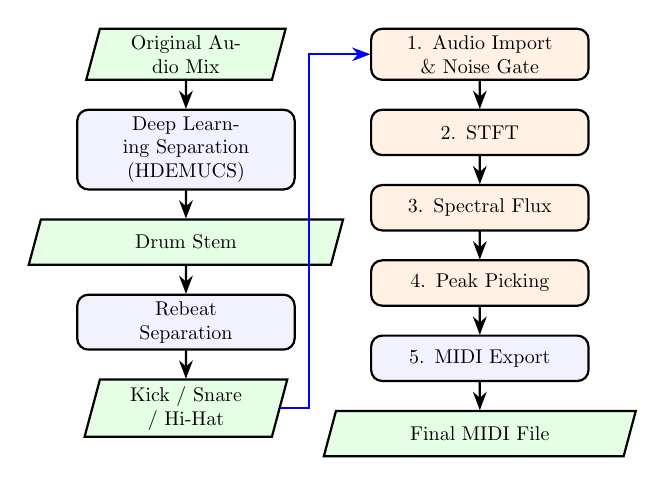
\begin{tikzpicture}[
    scale=0.72,
    transform shape,
    node distance=0.5cm and 1.2cm,
    process/.style={rectangle, draw=black, thick, rounded corners, text width=3.6cm, align=center, minimum height=0.8cm, fill=blue!5},
    algorithm/.style={rectangle, draw=black, thick, rounded corners, text width=3.6cm, align=center, minimum height=0.8cm, fill=orange!10},
    io/.style={trapezium, trapezium left angle=75, trapezium right angle=105, draw=black, thick, text width=2.8cm, align=center, minimum height=0.8cm, fill=green!10},
    arrow/.style={-{Stealth[scale=1.0]}, thick}
]

\node[io] (input) {Original Audio Mix};
\node[process, below=of input] (demucs) {Deep Learning Separation\\(HDEMUCS)};
\node[io, below=of demucs] (drumstem) {Drum Stem};
\node[process, below=of drumstem] (rebeat) {Rebeat\\Separation};
\node[io, below=of rebeat] (elements) {Kick / Snare / Hi-Hat};

\node[algorithm, right=1.6cm of input] (import) {1. Audio Import\\\& Noise Gate};
\node[algorithm, below=of import] (stft) {2. STFT};
\node[algorithm, below=of stft] (flux) {3. Spectral Flux};
\node[algorithm, below=of flux] (peaks) {4. Peak Picking};
\node[process, below=of peaks] (midi) {5. MIDI Export};
\node[io, below=of midi] (output) {Final MIDI File};

\draw[arrow] (input) -- (demucs);
\draw[arrow] (demucs) -- (drumstem);
\draw[arrow] (drumstem) -- (rebeat);
\draw[arrow] (rebeat) -- (elements);

\draw[arrow, blue] (elements.east) -- ++(0.5,0) |- (import.west);

\draw[arrow] (import) -- (stft);
\draw[arrow] (stft) -- (flux);
\draw[arrow] (flux) -- (peaks);
\draw[arrow] (peaks) -- (midi);
\draw[arrow] (midi) -- (output);

\end{tikzpicture}
\end{frame}

%------------------------------------------------
\begin{frame}{Object-Oriented Design}
    \begin{columns}[T]
        \begin{column}{0.48\textwidth}
            \begin{itemize}
                \item Strict \textbf{object-oriented design}
                \item Each processing step is implemented in a dedicated class
                \item Advantages:
                \begin{itemize}
                    \item modular structure
                    \item easier debugging
                    \item no global variables
                    \item better maintainability
                \end{itemize}
                \item Main classes:
                \begin{itemize}
                    \item \texttt{LoadAudioFile}
                    \item \texttt{LoadSTFT}
                    \item \texttt{SpectralFluxCalculator}
                    \item \texttt{PeakPicking}
                    \item \texttt{MidiExport}
                \end{itemize}
            \end{itemize}
        \end{column}
        \begin{column}{0.48\textwidth}
            \centering
            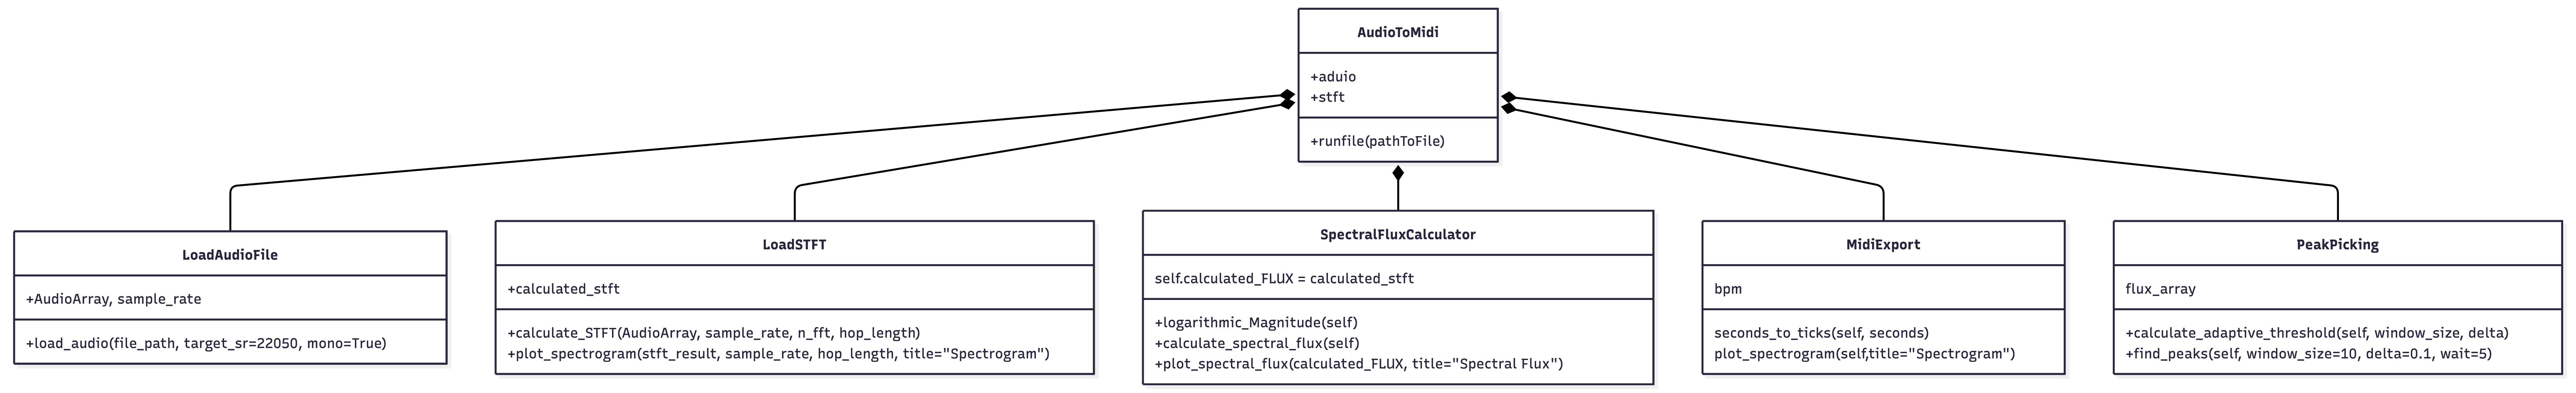
\includegraphics[width=\textwidth]{class_diagram.png}
        \end{column}
    \end{columns}
\end{frame}

%------------------------------------------------
\section{Audio Preprocessing}

\begin{frame}{Audio Import and Noise Gate}
    \begin{columns}[T]
        \begin{column}{0.5\textwidth}
            \begin{itemize}
                \item Audio is loaded with \textbf{librosa}
                \item Mono conversion and resampling to \textbf{44.1 kHz}
                \item A \textbf{noise gate} suppresses low-amplitude noise
                \item Threshold based on the \textbf{90th percentile} of the envelope
            \end{itemize}

            \[
            \text{env} = |\text{audio}|
            \qquad
            T = \text{percentile}(\text{env}, 90)
            \]

            \[
            x_{\text{gated}}[n] =
            \begin{cases}
                x[n], & |x[n]| \ge T \\
                0, & |x[n]| < T
            \end{cases}
            \]
        \end{column}
        \begin{column}{0.48\textwidth}
            \centering
            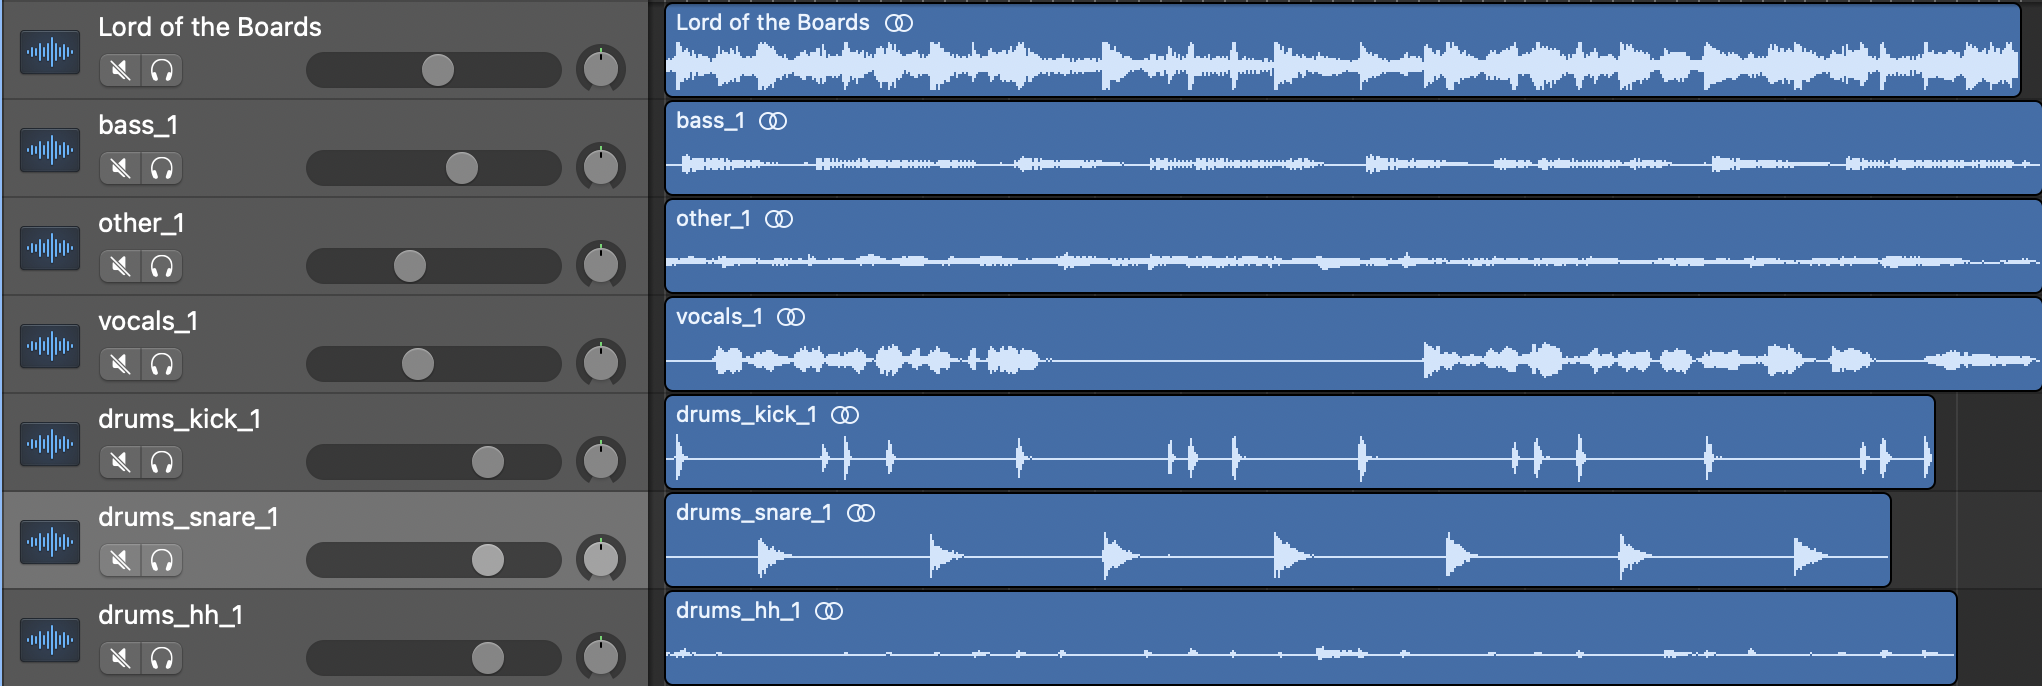
\includegraphics[width=\textwidth]{IsolatedAudio.png}
        \end{column}
    \end{columns}
\end{frame}

%------------------------------------------------
\section{STFT and Time-Frequency Analysis}

\begin{frame}{FFT and STFT}
    \begin{itemize}
        \item The \textbf{FFT} efficiently computes the Discrete Fourier Transform.
        \item Computational complexity is reduced from
        \[
        O(N^2) \rightarrow O(N \log N)
        \]
        \item For non-stationary audio, the signal is divided into overlapping frames.
        \item A window function is applied to each frame.
        \item This produces the \textbf{Short-Time Fourier Transform (STFT)}.
    \end{itemize}

    \[
    X(k)=\sum_{n=0}^{N-1}x(n)e^{-j2\pi kn/N}
    \]
\end{frame}

%------------------------------------------------
\begin{frame}{STFT: Principle and Spectrogram}
    \begin{itemize}
        \item The signal is split into short overlapping time frames.
        \item Each frame is multiplied by a window function.
        \item Then an FFT is calculated for every frame.
        \item The result is a time-frequency representation: the \textbf{spectrogram}.
    \end{itemize}

    \vspace{0.2cm}

    \[
    \mathbf{L} =
    \begin{bmatrix}
        1 & 4 & 1 & 6 \\
        3 & 2 & 2 & 1 \\
        1 & 5 & 3 & 6
    \end{bmatrix}
    \]

    \begin{itemize}
        \item Columns represent time frames.
        \item Rows represent frequency bins.
        \item This makes transient drum events visible over time.
    \end{itemize}
\end{frame}

%------------------------------------------------
\section{Spectral Flux and Onset Detection}

\begin{frame}{Spectral Flux}
    \begin{columns}[T]
        \begin{column}{0.48\textwidth}
            \begin{itemize}
                \item Drum hits create sudden increases in spectral energy.
                \item These increases are measured by the \textbf{spectral flux}.
                \item First, the logarithmic magnitude is calculated:
            \end{itemize}

            \[
            L(k)=\log_{10}(|X(k)|)
            \]

            \[
            \Delta L(k)=L_n(k)-L_{n-1}(k)
            \]

            \[
            F(n)=\sum_k |\Delta L(k)|
            \]
        \end{column}
        \begin{column}{0.48\textwidth}
            \centering
            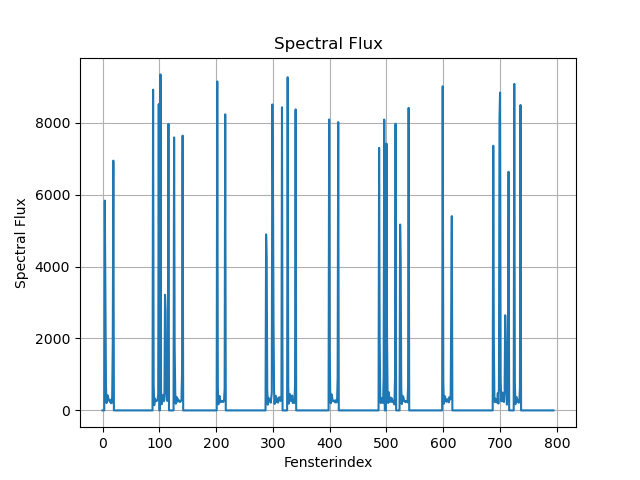
\includegraphics[width=\textwidth]{spectral_flux.png}
        \end{column}
    \end{columns}
\end{frame}

%------------------------------------------------
\begin{frame}{Spectral Flux Example with Matrices}
    \small
    Given the logarithmic magnitude spectrum:
    \[
    \mathbf{L} =
    \begin{bmatrix}
        1 & 4 & 1 & 6 \\
        3 & 2 & 2 & 1 \\
        1 & 5 & 3 & 6
    \end{bmatrix}
    \]

    The difference between consecutive frames is:
    \[
    \Delta \mathbf{L} =
    \begin{bmatrix}
        4 & 1 & 6 \\
        2 & 2 & 1 \\
        5 & 3 & 6
    \end{bmatrix}
    -
    \begin{bmatrix}
        1 & 4 & 1 \\
        3 & 2 & 2 \\
        1 & 5 & 3
    \end{bmatrix}
    =
    \begin{bmatrix}
        3 & -3 & 5 \\
        -1 & 0 & -1 \\
        4 & -2 & 3
    \end{bmatrix}
    \]

    Summing the absolute values column-wise gives:
    \[
    \mathbf{F} =
    \begin{bmatrix}
        |3|+|{-1}|+|4| \\
        |{-3}|+|0|+|{-2}| \\
        |5|+|{-1}|+|3|
    \end{bmatrix}
    =
    \begin{bmatrix}
        8 \\
        5 \\
        9
    \end{bmatrix}
    \]
\end{frame}

%------------------------------------------------
\begin{frame}{Half-Wave Rectification}
    \begin{columns}[T]
        \begin{column}{0.48\textwidth}
            \begin{itemize}
                \item Only \textbf{positive} energy changes are relevant.
                \item Negative values are discarded.
            \end{itemize}

            \[
            F_{\text{rect}}(n)=\max(0, F(n))
            \]

            \begin{itemize}
                \item This emphasizes attack transients.
                \item It improves onset detection for percussive sounds.
            \end{itemize}
        \end{column}
        \begin{column}{0.48\textwidth}
            \centering
            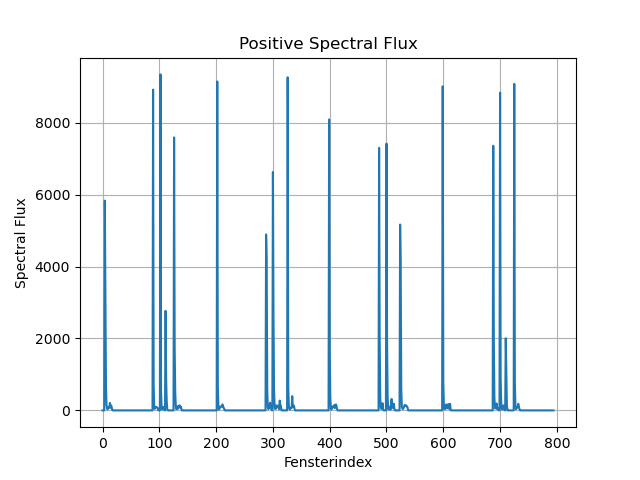
\includegraphics[width=\textwidth]{positive_spectral_flux.png}
        \end{column}
    \end{columns}
\end{frame}

%------------------------------------------------
\section{Peak Picking}

\begin{frame}{Adaptive Threshold and Peak Picking}
    \begin{itemize}
        \item A fixed threshold is not robust enough for varying audio levels.
        \item Therefore, an \textbf{adaptive threshold} is used.
        \item It is based on a moving average:
    \end{itemize}

    \[
    y[n] = \frac{1}{N}\sum_{k=-\lfloor N/2 \rfloor}^{\lfloor (N-1)/2 \rfloor} x[n+k]
    \]

    \begin{itemize}
        \item An additional offset avoids detections from the noise floor.
        \item A valid onset must satisfy:
        \begin{enumerate}
            \item above threshold,
            \item local maximum,
            \item enough distance to the previous onset.
        \end{enumerate}
    \end{itemize}
\end{frame}

%------------------------------------------------
\begin{frame}{Peak Picking Visualization}
    \centering
    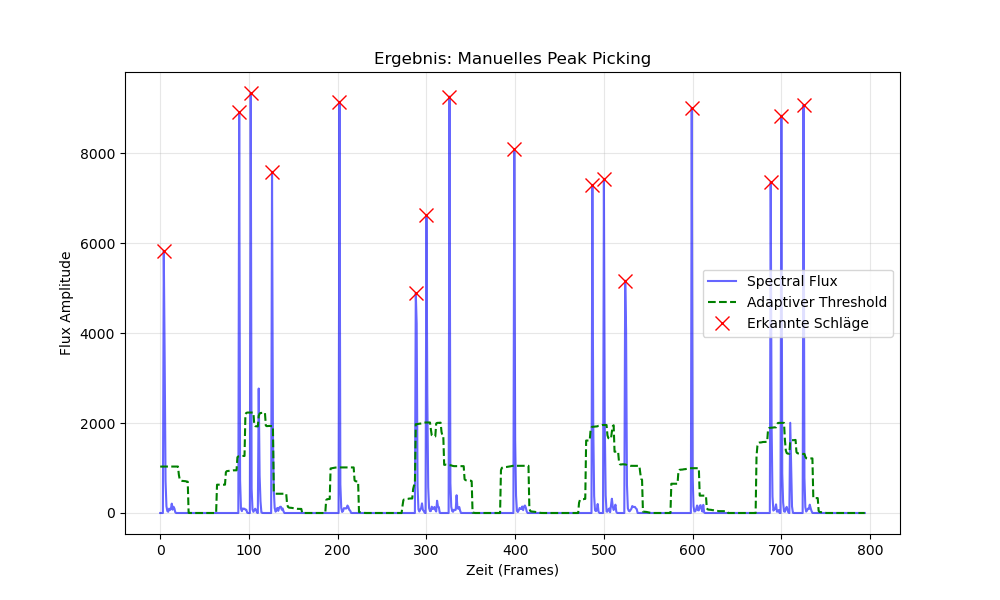
\includegraphics[width=0.9\textwidth]{peak_picking.png}

    \vspace{0.3cm}
    \begin{itemize}
        \item Peaks are selected only if they exceed the adaptive threshold.
        \item Debouncing prevents multiple detections of the same hit.
    \end{itemize}
\end{frame}

%------------------------------------------------
\begin{frame}[fragile]{Peak Picking Implementation}
\begin{lstlisting}
def find_peaks(self, window_size, wait):
    thresholds = self.calculate_adaptive_threshold(window_size)
    found_peaks = []
    last_peak_index = -wait

    for i in range(1, len(self.flux) - 1):
        current_val = self.flux[i]

        if current_val > thresholds[i]:
            if current_val > self.flux[i-1] and current_val > self.flux[i+1]:
                if (i - last_peak_index) > wait:
                    found_peaks.append(i)
                    last_peak_index = i

    self.onsets = np.array(found_peaks)
    return self.onsets
\end{lstlisting}
\end{frame}

%------------------------------------------------
\section{MIDI Export}

\begin{frame}{MIDI Export}
    \begin{itemize}
        \item Detected onset frames are converted into MIDI events.
        \item Required parameters:
        \begin{itemize}
            \item onset frames,
            \item sample rate,
            \item hop length,
            \item BPM.
        \end{itemize}
        \item Output:
        \begin{itemize}
            \item \textbf{multi-track MIDI file}
            \item routed to \textbf{MIDI channel 10}
        \end{itemize}
        \item General MIDI mapping:
        \begin{itemize}
            \item Kick: 36
            \item Snare: 38
            \item Closed Hi-Hat: 42
        \end{itemize}
    \end{itemize}
\end{frame}

%------------------------------------------------
\section{Conclusion}

\begin{frame}{Conclusion and Outlook}
    \begin{itemize}
        \item The system can generate usable MIDI drum patterns from audio.
        \item It combines:
        \begin{itemize}
            \item AI-based source separation
            \item classical DSP methods
            \item rule-based onset detection
        \end{itemize}
        \item Main limitations:
        \begin{itemize}
            \item imperfect source separation
            \item overlap between drum components
            \item noise in extracted stems
        \end{itemize}
        \item Future work:
        \begin{itemize}
            \item improved separation models
            \item more robust onset detection
            \item automatic tempo estimation
        \end{itemize}
    \end{itemize}
\end{frame}

%------------------------------------------------
\begin{frame}{References}
\footnotesize
\begin{thebibliography}{99}

\bibitem{librosa}
Librosa Developers, \emph{Librosa documentation}. \url{https://librosa.org/doc/main/index.html}

\bibitem{matplotlib}
Matplotlib Developers, \emph{Matplotlib Documentation}. \url{https://matplotlib.org/}

\bibitem{numpy}
NumPy Developers, \emph{NumPy Documentation}. \url{https://numpy.org/devdocs/index.html}

\bibitem{pytorch}
PyTorch Developers, \emph{PyTorch Documentation}. \url{https://pytorch.org/}

\bibitem{rebeat}
Rebeat Developers, \emph{Rebeat App and documentation}. \url{https://rebeatapp.com/}

\bibitem{scipy}
SciPy Developers, \emph{Scipy Documentation}. \url{https://docs.scipy.org/doc/scipy/index.html}

\bibitem{torchaudio}
Torchaudio Developers, \emph{Hybrid Demucs Tutorial}. \url{https://docs.pytorch.org/audio/2.8/tutorials/hybrid_demucs_tutorial.html}

\bibitem{mido}
Mido Developers, \emph{Mido Documentation}. \url{https://mido.readthedocs.io/en/stable/}

\end{thebibliography}
\end{frame}

%------------------------------------------------
\begin{frame}
    \centering
    \Huge Thank you for your attention
\end{frame}

\end{document}